\pagebreak
\section{3D gedruckte Komponenten}\label{sec:gehaeuse}
Für das Unterbringen des Mikroprozessors und der Sensoren werden zwei verschiedene Gehäusevarianten verwendet. Dieses Kapitel beschäfftigt sich mit deren Entwurf, sowie dem Entwurf des Adapters, mit welchem die Windfahne und das Anemometer an der Wetterstation befestigt sind.

Für den Entwurf der Komponenten wurde die Studentenversion von Autocad Fusion 360 verwendet.

\subsection{Hauptgehäuse}\label{sec:ge_haupt}
Das Hauptgehäuse beinhaltet das Mikroprozessor-Board mit den zwei aufsteckbaren Platinen sowie den Sensoren. Drei der Sensoren befinden sich nicht im Hauptgehäuse (s. Kap.~\ref{sec:ge_neben}).

Das Gehäuse besteht aus zwei Teilen (s. Abb. \ref{fig:main}), dem Hauptteil (links) und dem Deckel (rechts). Das STM8 Nucleo Board wird von drei Pins in Position gehalten (s. Abb.~\ref{fig:main},~\ref{fig:main_top}). In der Vorderseite befinden sich zwei Aussparungen (s. Abb.~\ref{fig:main_front}). Über die Rechte ist der USB-Port des Mikroprozessor-Boards erreichbar. Hinter der Linken befindet sich der Motortreiber, welcher auf einer leicht erhöhten Plattform plaziert wird (s. Abb.~\ref{fig:main_top}). Über die Aussparung an der rechten Seite kann die SD-Karte erreicht werden. Die Aussparung an der hinteren Seite wird verwendet, um alle externen Komponenten mit dem Mikroprozessor-Board zu verbinden.

Im Deckel befinden sich drei Löcher, in welche Status-LEDs untergebracht werden.

Das Hauptteil und der Deckel werden lediglich aufeinander gesteckt. Bedingt durch die Geometrie entsteht ein relativ fester Halt. Optional können die Komponenten über die vier Aussparungen an den Seiten, mit beispielsweise Kabelbindern, zusätzlich gesichert werden.
\begin{figure}[H]
  \centering
  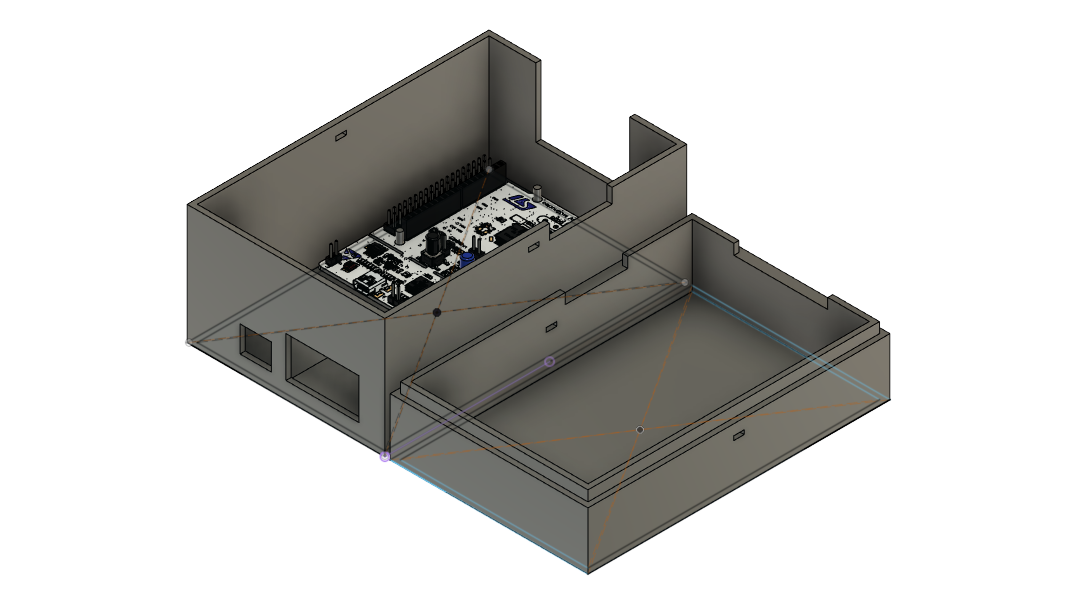
\includegraphics[width=\textwidth]{./img/ST_MainBodyv13}
  \caption{Hauptgehäuse}\label{fig:main}
\end{figure}
\begin{figure}[H]
  \centering
  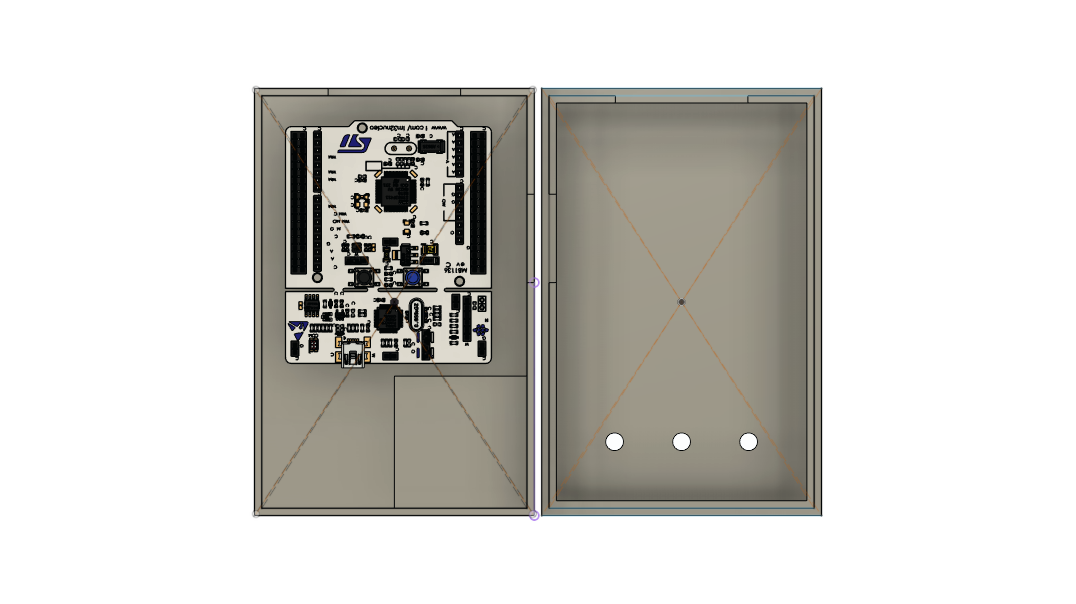
\includegraphics[width=\textwidth]{./img/ST_MainBodyv13_top}
  \caption{Hauptgehäuse, Ansicht von oben}\label{fig:main_top}
\end{figure}
\begin{figure}[H]
  \centering
  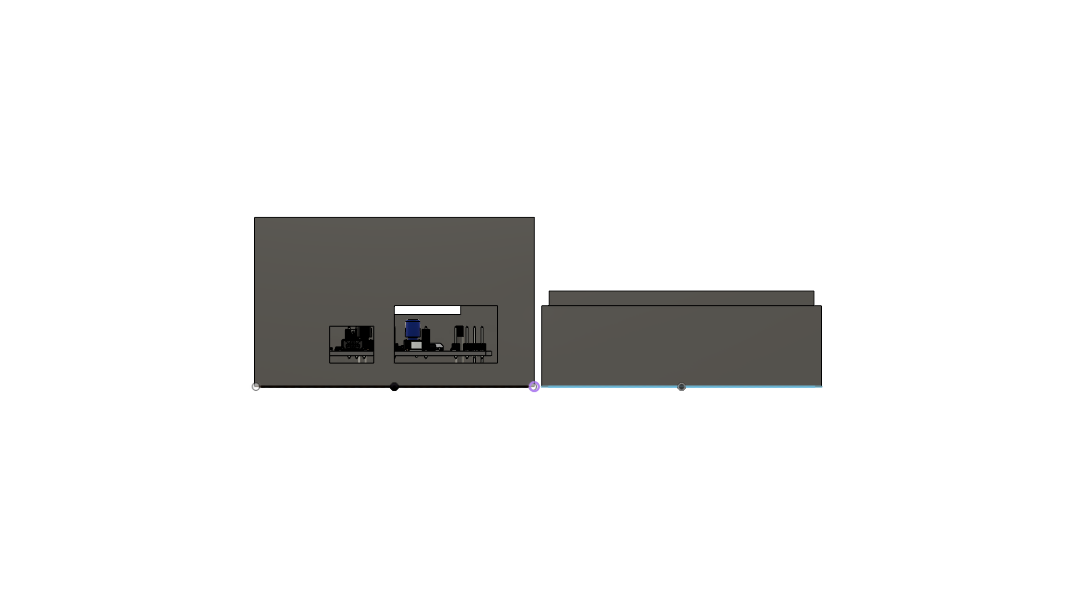
\includegraphics[width=\textwidth]{./img/ST_MainBodyv13_front}
  \caption{Hauptgehäuse, Ansicht von vorne}\label{fig:main_front}
\end{figure}
\subsection{Nebengehäuse}\label{sec:ge_neben}
Es wird jeweils ein Nebengehäuse für folgende Sensoren verwendet:
\begin{itemize}
\item der Neigungssensor, welcher an der Unterseite des Solarpanels befestigt werden muss
\item der GPS-Empfänger, welcher für besseren Empfang am oberen Ende der Wetterstation befestigt wird
\item das Kompass-Modul, welches empfindlich auf elektro-magnetische Störungen reagiert und aus diesem Grund auch am oberen Ende der Wetterstation untergebracht wird (auf der Seite gegenüber des GPS-Empfängers)
\end{itemize}
Die Nebengehäuse bestehen aus zwei Teilen, welche aufeinandergesteckt werden und zusätzlich, optional, mittels Kabelbinder gesichert werden (s. Abb.~\ref{fig:secondary},~\ref{fig:secondary_front}).

Die Nebengehäuse werden mit einer Schraube und einer Mutter am Aluminium-Profil der Wetterstation befestigt (s.Abb.~\ref{fig:secondary_top}). Das Nebengehäuse, welches sich auf dem Solarpanel befindet, kann nicht geschraubt werden und wird entsprechend mit Klebstoff befestigt.

Die runden Aussparungen an der linken und rechten Seiten dienen dem Durchführen von benötigten Leitungen.
\begin{figure}[H]
  \centering
  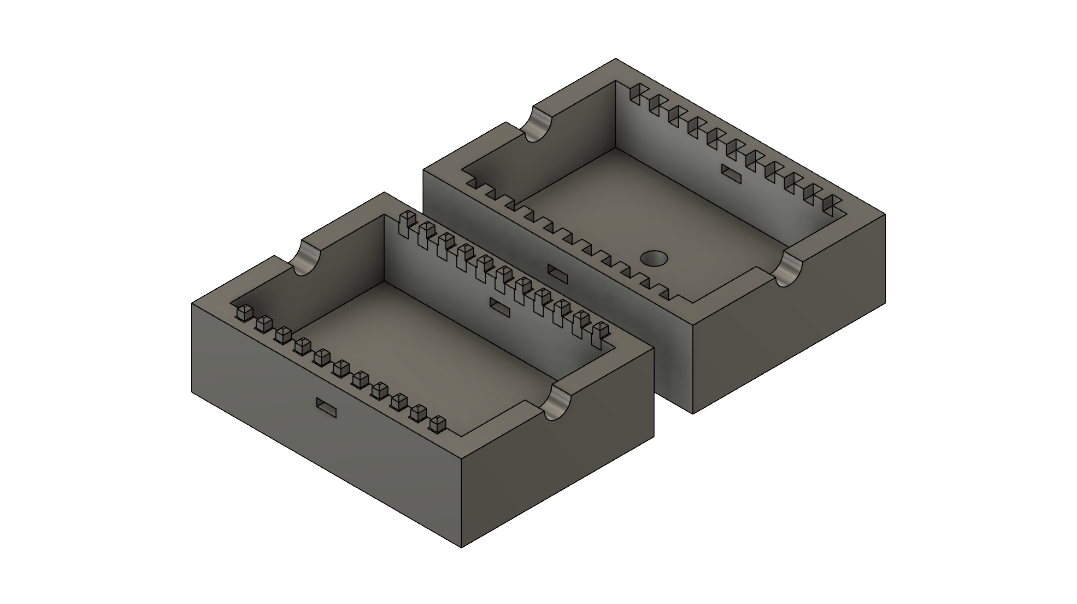
\includegraphics[width=\textwidth]{./img/ST_Halterv5}
  \caption{Nebengehäuse}\label{fig:secondary}
\end{figure}
\begin{figure}[H]
  \centering
  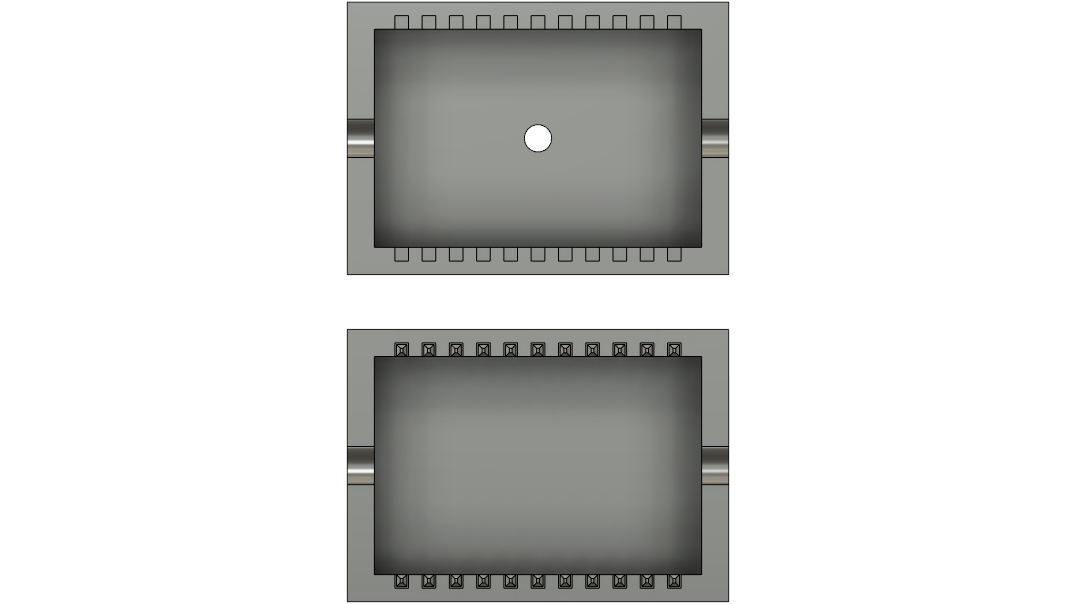
\includegraphics[width=\textwidth]{./img/ST_Halterv5_top}
  \caption{Nebengehäuse, Ansicht von oben}\label{fig:secondary_top}
\end{figure}
\begin{figure}[H]
  \centering
  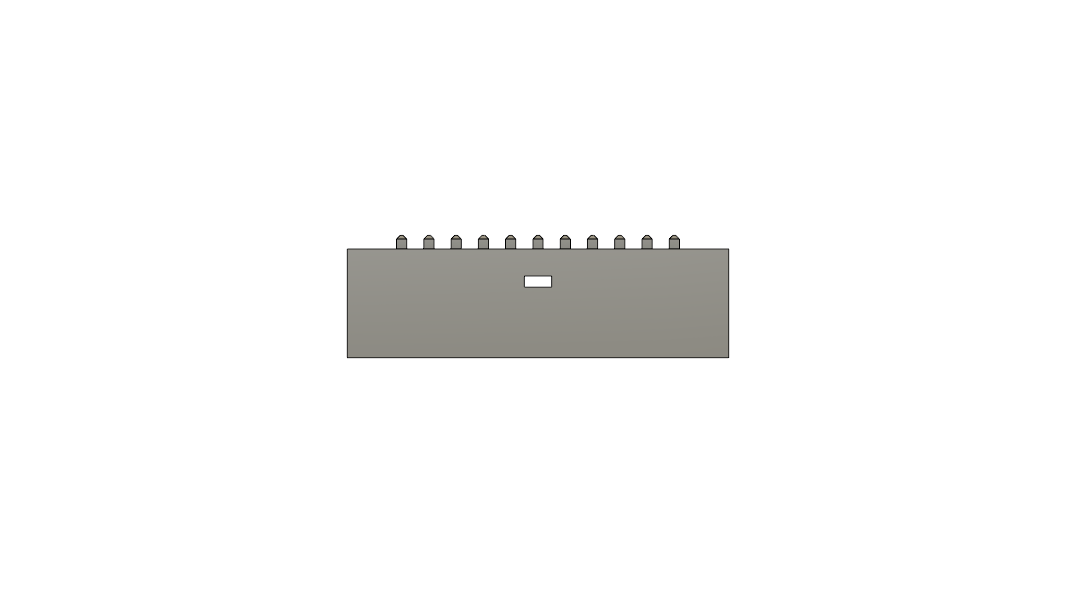
\includegraphics[width=\textwidth]{./img/ST_Halterv5_front}
  \caption{Nebengehäuse, Ansicht von vorne}\label{fig:secondary_front}
\end{figure}
\subsection{Adapter}\label{sec:ge_adapt}
Der Adapter wird verwendet, um eine feste Verbindung zwischem dem Alluminium-Profil der Wetterstaion und dem Mast mit Windfahne und Anemometer herzustellen.

Die Verbindung zur Wetterstation erfolgt durch Stecken der vier trapez-förmigen Steckkontakte am unteren Ende des Adapters (s. Abb.~\ref{fig:adapter},~\ref{fig:adapter_front}).

Der Mast wird von oben auf die angepasste Aussparung gesteckt. Optional kann dieser mittels Schraubverbindung fixiert werden (s. Abb.~\ref{fig:adapter},~\ref{fig:adapter_top}).
\begin{figure}[H]
  \centering
  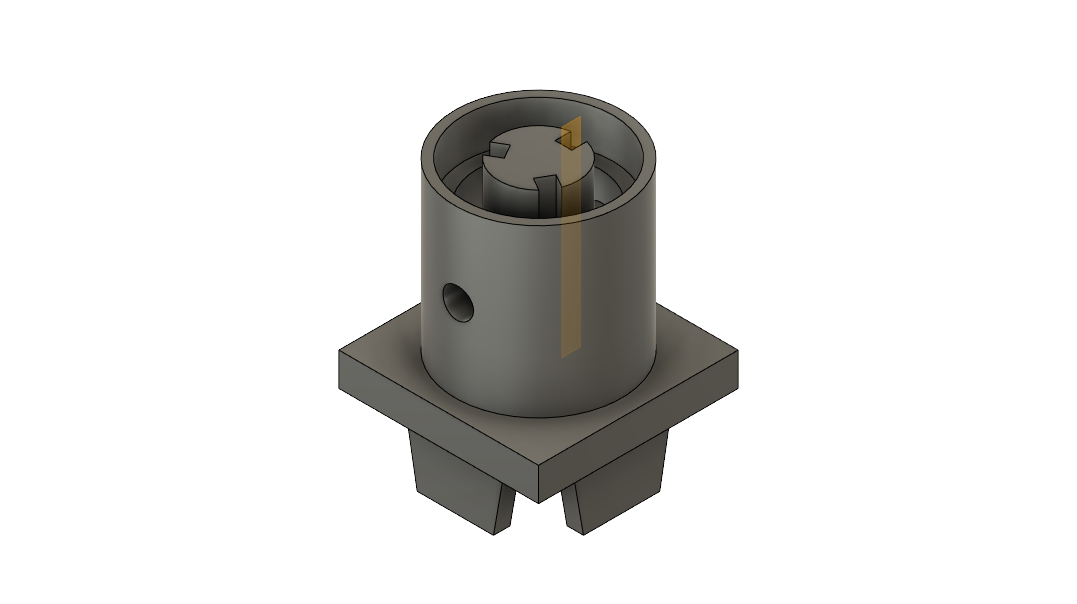
\includegraphics[width=\textwidth]{./img/ST_Adapterv4}
  \caption{Adapter}\label{fig:adapter}
\end{figure}
\begin{figure}[H]
  \centering
  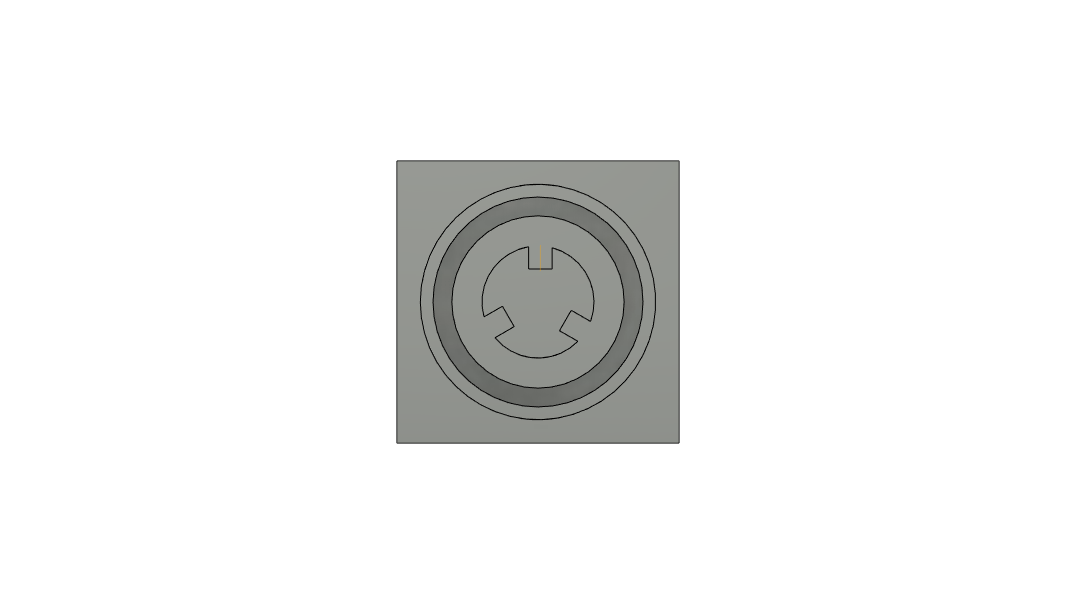
\includegraphics[width=\textwidth]{./img/ST_Adapterv4_top}
  \caption{Adapter, Ansicht von oben}\label{fig:adapter_top}
\end{figure}
\begin{figure}[H]
  \centering
  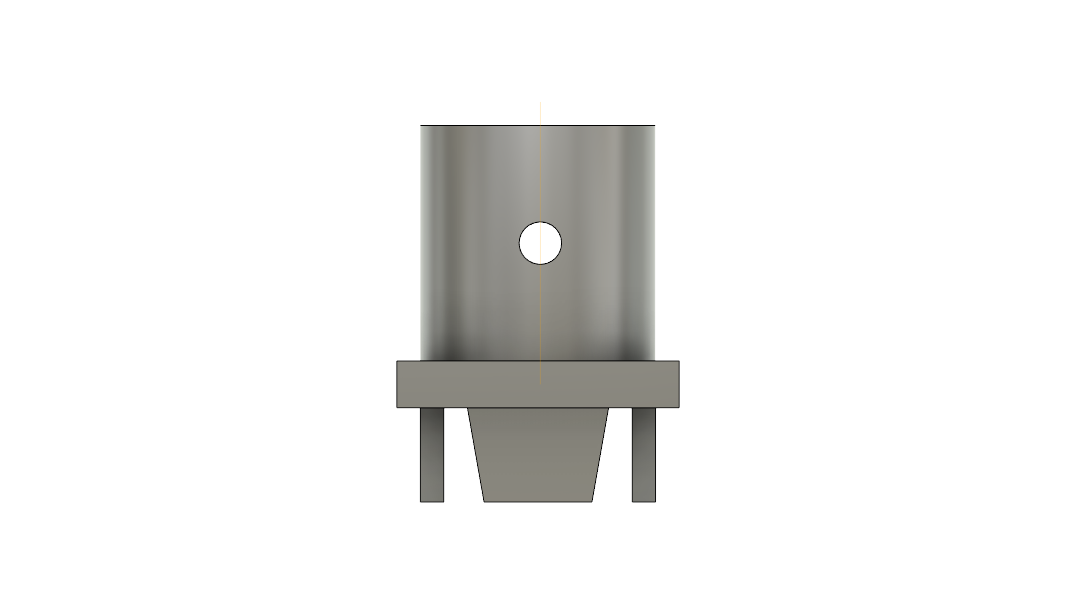
\includegraphics[width=\textwidth]{./img/ST_Adapterv4_front}
  \caption{Adapter, Ansicht von vorne}\label{fig:adapter_front}
\end{figure}
\subsection{Herstellung}\label{sec:ge_herst}
Alle Komponenten wurden in PLA mit einer Schichtdicke von \SI{0.2}{\milli\meter} gedruckt. Es wurden zwei bis drei Top-, Buttom- und Wandschichten gedruckt. Da die Komponenten keine großen Kräfte aushalten müssen wurden sie lediglich mit einem Infill von \SI{10}{\percent} bis \SI{20}{\percent} gedruckt.
%%% Local Variables:
%%% mode: latex
%%% TeX-master: "../termpaper"
%%% End:
